\section{Multi-Authority Attribute-Based Encryption}
In the following sections, the different sub topics of \textit{Multi-Authority Attribute-Based Encryption} (\ac{MA-ABE}) will be described, analyzed given all the requirements and finally evaluated based on their performance and scalability. 

\subsection{Introduction Into Multi-Authority Attribute-Based Encryption}
2007 was the first year were Chase \cite{chase2007multi} introduced a working \ac{MA-ABE} scheme. In her paper she describes the process on how to derive a multi-authority attribute-based encryption scheme from the single authority scheme. Her proposal focused on interpolation and the fact that no under defined linear equation system could definitely be solved as the main security assumption\footnote{\ac{LSSS} matrix are based on the same assumption.}.  

To ensure collusion resistance, each user is given blinded attribute private keys so that when used on decryption the plain text is still blinded with the user specific identifier. Using pairings (bilinear maps, section \ref{sec:bilinearmappings}) this identifier can be substituted and the plain text gets revealed. 

Chases scheme had two major disadvantages which were not addressed in her initial scheme. First, the \ac{CA} had global decryption power. That was due to the bootstrapping of the different AAs and users. The CA had to give the right seeds and global parameter to each AA to make sure that each decryption of a cipher text results in a blinded plain text that can only be decrypted using attribute keys of the same user. If this would not be the case users could easily collude. 

% That was due to the fact that it needed to issue each \ac{AA} a specific seed so that, on using this seed in a pseudo random generator, the \ac{CA} knew what random value would be calculated. This information is used to precompute the users secret key so that when later combined with the secret attribute keys, it resolves in the correct plain text. This was important since the CA, in comparison to the AA, was defined as the trusted authority. So the cipher text need this extra security layer.  

Chase improved her scheme 2009 in \cite{chase2009improving} to deescalate the global decryption power of the CA. Now all \ac{AA}s will do a $n$-party key exchange to agree on $n$ secret seeds from which the personal initial seed can be calculated. This results in the fact that no AA know the whole master secret but only its required secret seeds. Agreeing on a well known value the \ac{CA} was no longer required and as long $N-2$ \ac{AA}s are not colluding with each other the master secret remains secure. 

The other disadvantage, which is also still present in the updated scheme, is that no new \ac{AA} could be added after system initialization since it would trigger a new system bootstrap and distribution of the master secret. 

The lack of adding new attributes and the missing revocation scheme makes Chases scheme impractical for further evaluations but gives a good introduction the challenges of the \ac{MA-ABE} schemes.

\subsection{Hierarchical \ac{ABE}}
\label{sec:HABE}

\begin{figure*}[!ht]
\centering
    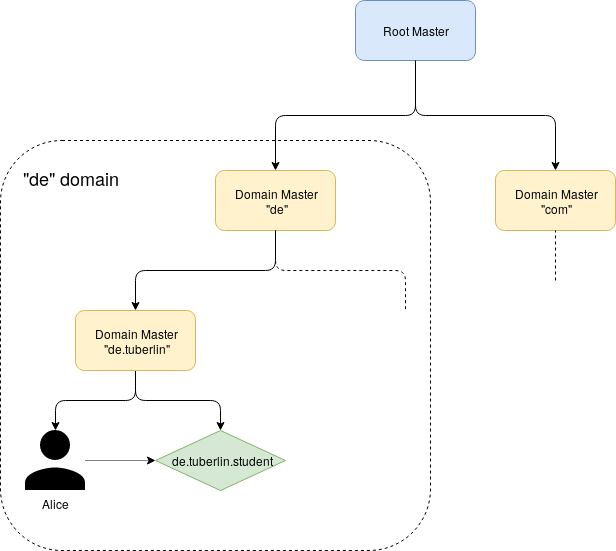
\includegraphics[width=0.7\linewidth]{img/HABE.png}
    \caption{Structure of hierarchical attribute-based encryption systems}
    \label{fig:habe}
\end{figure*}

\textit{Hierarchical Attribute-Based Encryption} (\ac{HABE}) is based of the idea of key and decryption power delegation. If a private key exist that have a certain access power, it is possible for the key holder to delegate a subset of his access power to a new instance. By nature follows a hierarchical structure where each user could administrate an own subdomain. Many use cases for cloud computing as well as cloud storage system emerged \cite{Wang:2010:HAE:1866307.1866414}. While some works also take revocation into design a crucial requirement is still missing:  The domain master has always global decryption power. 

As displayed in figure \ref{fig:habe}, which is based on the approach by Wang \textit{et. al.} \cite{wang2011hierarchical}, the root master summarized the global decryption power of the system and can set up new domain masters (attribute authorities). They on the other hand can delegate a subset of their decryption power to a sub domain master. Each domain master can administer users and attributes.

"Hierarchical Attribute-based Encryption for Fine-grained Access Control in Cloud Storage Services" \cite{Wang:2010:HAE:1866307.1866414} formalized this approach using \ac{CP-ABE}, which was later extended in "Hierarchical attribute-based encryption and scalable user revocation for sharing data in cloud servers" \cite{wang2011hierarchical}. While this implementation serves with a revocation scheme it depends on an access policy in disjunctive normal form (\ac{DNF}). Any boolean formula can be transferred into DNF but sometimes this might enforce negation. Since Wang \textit{et. al.} \cite{wang2011hierarchical} did not provide any negation mechanism, this ABE scheme is limited in expressivenss.

\subsection{Decentralized Attribute-Based Encryption}
\label{sec:DABE}
In contrast to HABE stands \textit{decentralized attribute-based encryption} (\ac{DABE}) which is structured around the idea of having a peer network of authorities and user. No entity has a global view of the system and no entity is in charge of bootstrapping AAs. This ecosystem is self sustaining so that each entity can become an \ac{AA} if needed and start issuing new attributes to users. 

However, some form of centralization must still be present. The global parameters, for example , need to be known to each new entity and each user still need to get a unique global identifier assigned to prevent collusion. Also attributes need to be synchronized since the set of attribute identifier need to be non-intersecting across different domains. While not being a limitation it is rather a challenge to enable global communication and achieve global synchronization across the network. Such a distributed system was first formalized in "Decentralizing attribute-based encryption" \cite{lewko2011decentralizing}. 

Revocation in a distributed setting remains an open issue. Since no central authority has a global view over the users, no authority can be in charge of revoking them. An authority could revoke its issued attributes but only in an indirect fashion since decentralized systems always have to take into account that nodes do not have to be online all the time. If an authority would go offline as soon at it received the revocation request the revocation procedure would never trigger. 

Cui and Deng showed in \cite{cui2016revocable} that a DABE system with indirect revocation could exist. Each key and ciphertext get a liveness assigned which make them valid for a certain time period. After this time period expires all keys need to be reissued by each \ac{AA}. Indirect revocation happens by simply excluding the user from reissuing certain attribute keys. This system is implemented in the comparison in \ref{sec:ma-comparison}.

However, question remains if such a system would be practically applicable in the real world since each ciphertext need to be reuploaded and each attribute keys need to be redistributed in each time period. Until now no direct revocation DABE was developed.

\subsection{Efficient Data Access Control For Multi-Authority Cloud Storage}
The most explored field in \ac{MA-ABE} is the \textit{Efficient Data Access Control for Multi-Authority Cloud Storage Systems} (\ac{DAC-MACS}) family \cite{yang2013dac}). First introduced by Yang \textit{et. al.} 2013 it describes an efficient, revocable \ac{MA-ABE} scheme based on \ac{CP-ABE} which uses proxy encryption on decryption and reencryption to make the scheme more efficient. 

Proxy de-/reencryption, as demonstrated in the litrature by \cite{yang2013dac}, \cite{wu2017security}, \cite{li2017two} and \cite{wang2011hierarchical}, is a technique where the a server helps the user on decryption to reduce the computationally intensive work. It is motivated by the fact that mobile devices often don't have much computing resources so the server helps the clients on decryption. The main idea is that the server does the preprocessing of the encrypted text given attribute keys by the user. Impotent to note is that the server will have no knowledge about the plain text since the preprocessed cipher text is still encrypted with the users public key.

DAC-MACS also features a large attribute universe, adding \ac{AA}s on the running system and deescalates the global decryption power of the \ac{CA}. In sort \ac{DAC-MACS} satisfy all the non-optional requirements.

In contrast to Chases scheme, DAC-MACS eliminates the need for the global decryption power of the \ac{CA} by issuing $k$ ciphertexts: One per \ac{AA}. \footnote{If the ciphertext does not require any attributes of an specific authority it does not have to create a ciphertext for this domain.} It does not require any coordination between authorities which enables to add new \ac{AA}s at runtime without recreating the user keys. This scheme also includes features for efficient revocation while it claims to maintain forward and backward secrecy.

\ac{DAC-MACS} is not collusion resistance on attribute revocation under the active attack model. The scheme \ac{NEDAC-MACS} (New-Extended \ac{DAC-MACS}) shows and solves this vulnerability \cite{wu2017security}. Recent studies introduce a more efficient, scalable and secure approaches such as \ac{MAACS} \cite{li2016secure} and \ac{TF-DAC-MACS} (Two-Factor \ac{DAC-MACS})\cite{li2017two}. 

All the \ac{DAC-MACS} schemes are structured in roughly the same way. They usually describe six different entities:

\begin{enumerate}
	\item \textbf{Certificate/Central Authority (\ac{CA});} The purpose of the \ac{CA} is to issue user their global identifier (\ac{GID}). Further, it bootstraps the different \ac{AA}s. The \ac{CA} remains trusted but do not have any decryption power in the system. 
	\item \textbf{Attribute Authority (\ac{AA});} An attribute authority administers its own domain. Here it issues attributes and their respective private key to the user. They only accept a user if his \ac{GID} is signed by the \ac{CA}. 
	On revocation the AA will need to update the users secret keys as well as the ciphertext encrypted with the revoked attribute key. \ac{AA}s are assumed to be honest-but-curious.
	\item \textbf{Server;} The purpose of the server is to help the user with proxy re- and decryption. If an \ac{AA} broadcasts a revocation of an attribute, the server downloads all related ciphertexts from the \ac{CSP} to update them with the new attribute. 
	Further, the user may give the server his attribute private keys so that the server can precompute the ciphertext. The thread model for the server is honest-but-curious. Please note, that the \ac{CA} and the server are two separated entities that do not cooperate.
	\item \textbf{Cloud Storage Provider (\ac{CSP});} The cloud storage provider are assumed to be untrusted but they still follow the protocol. That’s why they only receive encrypted data. They only purpose is to store the ciphertext and make them permanentally available. No authentication checks are needed.
	\item \textbf{Users;} Users exist in two groups: Revoked and non-revoked. Non-revoked users try to collude with each other to get a higher level of decryption power. They download the files of the \ac{CSP} and try to decrypt them. Only if they attribute set matches the policy of the ciphertext they will be able to decrypt the file. 
	Revoked users, on the other hand, try to still decipher ciphertext. In some cases they try to collude with non-revoked user to intercept the key update key to restore their decryption rights. 
	User are in general untrusted.
	\item \textbf{Data Owner;} The data owner are users who want to encrypt content with a specific access policy. To do so they use the public available public attribute keys pinned on the bulletin board of the respective \ac{AA}. Data owner do not have to know anything about the receiving user or user groups in the system. After encryption they update the encrypted content to the \ac{CSP}.
\end{enumerate} 

For the comparison we will use the charm implementation of DAC-MACS \cite{yang2013dac}.

\ac{TF-DAC-MACS} counts as the most advanced \ac{DAC-MACS} scheme providing non global decryption power, secure revocation channels and both backward and forward secrecy. In addition \ac{TF-DAC-MACS} introduces the two-factor authentication. Data owner can issue and revoke \textit{authentication keys} to and from other users. This adds an additional layer of security. In total \ac{TF-DAC-MACS} achieves still better performance then the other \ac{DAC-MACS} schemes providing constant decryption and encryption overhead. 
To compare the TF-DAC-MACS with the others we will implement TF-DAC-MACS from scratch. 

\subsection{Comparison}
\label{sec:ma-comparison}
\begin{table*}[!ht]
\centering
\begin{tabular}{l 					| l 									| l 									| l 					| l}
									& \thead{LTXWC 16 \cite{li2017two}\\(TF-DAC-MACS)} & \thead{YJ 14 \cite{yang2013dac}\\(DAC-MACS)} & \thead{LW 14\cite{wang2011hierarchical} \\ (HABE)}	& \thead{CD 16 \cite{cui2016revocable}\\(DABE)} \\
\hline
\thead{Scheme}						& \makecell{CP\\(DAC-MACS\\ without proxy \\ 
									  decryption, 
									  with \\ two-factor \\ authentication)} & \makecell{CP\\(DAC-MACS \\ 
									  										  with proxy \\ decryption)} 			& \makecell{CP\\(Hierar-\\chical)} 		& \makecell{CP\\(Decent-\\ralized)}		\\ 
\hline
\thead{Revocation}					& Direct 								& Direct 								& Direct 				& Indirect					\\
\hline
\thead{Security\\scheme}				& \makecell{Bilinear\\maps}			& \makecell{Bilinear\\maps}				& \makecell{Bilinear\\maps}& \makecell{Bilinear\\maps} 			\\
\hline
\thead{Expression of \\ access policy} & n-of-n threshold					& LSSS		 							& DNF 					& LSSS  				\\ 
\end{tabular}
\caption{Scheme description. }
\label{tab:comparison_ma_abe_overview}
\end{table*}
\begin{table*}[!ht]
\centering
\begin{tabular}{l 	| l										| l 									| l 					| l}
					& \thead{LTXWC 16\\(TF-DAC-MACS)\cite{li2017two}} & \thead{YJ 14\\(DAC-MACS)\cite{yang2013dac}} & \thead{LW 14\\ (HABE)\cite{wang2011hierarchical}}	& \thead{CD 16\\(DABE)}\cite{cui2016revocable} \\
\req{C1}			& Yes									& No 									& Yes 					& Yes 						\\
\req{C2}			& Yes									& Yes 									& Yes 					& Yes 						\\ 
\req{C3}			& Yes									& Yes 									& No 					& Yes 						\\ 
\req{C4}			& Yes									& Yes 									& No 					& Yes 						\\ 
\req{C5}			& Yes									& Yes 									& Yes 					& Yes 						\\ 
\req{C6}			& Yes 									& Yes 									& Yes					& Yes						\\
\req{C7}			& Yes									& Yes 									& No 					& Yes 						\\
\req{C8}			& Yes									& Yes									& Yes					& Yes-						\\
\req{O1}			& No 									& No 									& No 					& No 						\\
\req{O2}			& No 									& Yes									& Yes					& Yes						\\
\end{tabular}
\caption{Requirements comparison of the implemented schemes}
\label{tab:ma_abe_comparisons}
\end{table*}


\begin{figure*}[!ht]
\centering
    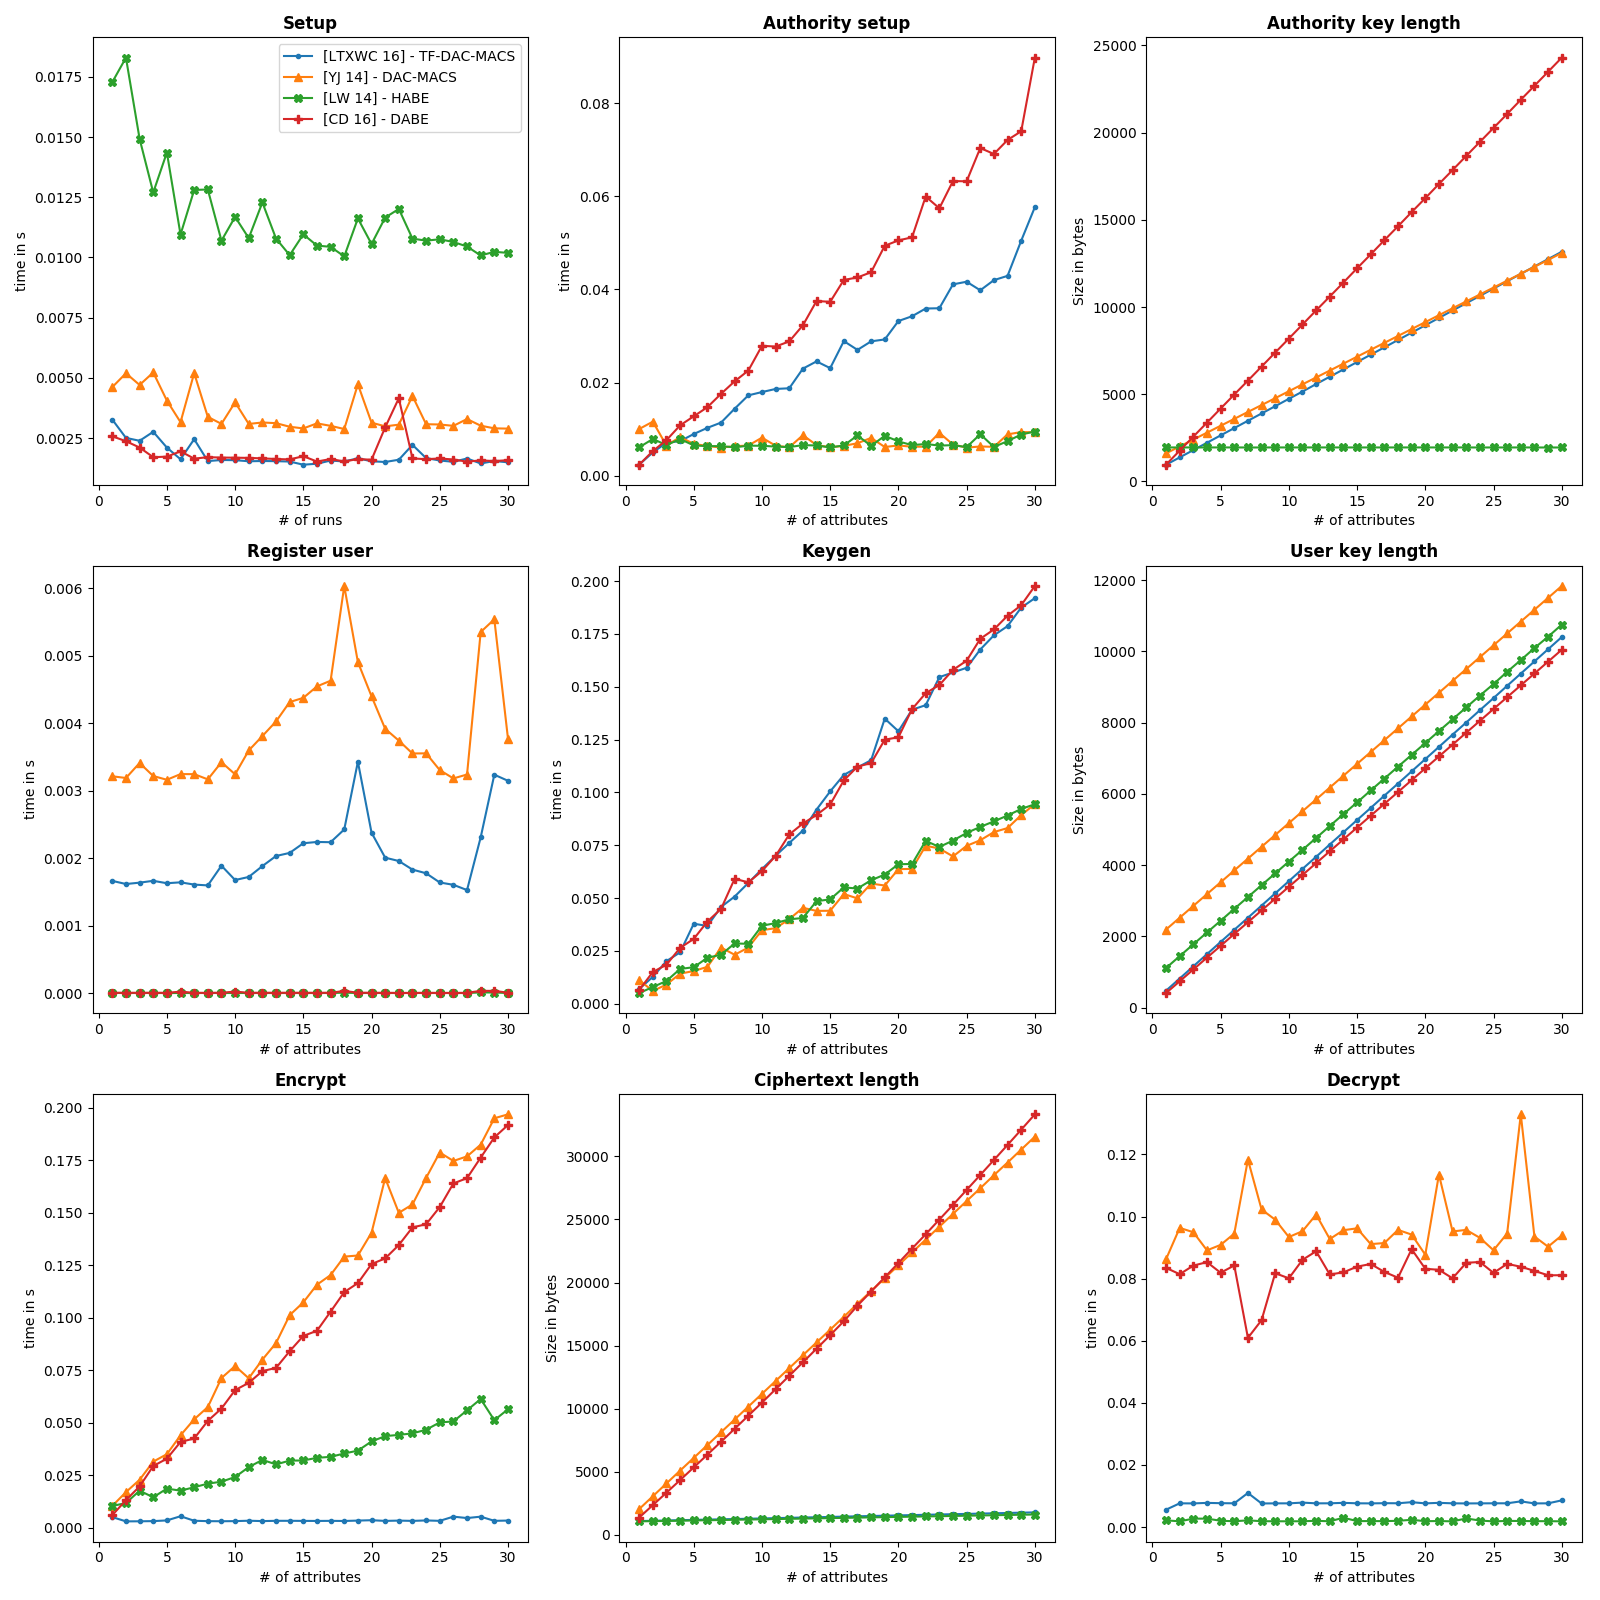
\includegraphics[width=1\linewidth]{img/maabe_comparisons.png}
    \caption{Performance and scalability comparison}
    \label{fig:maabe_comparison}
\end{figure*}

To compare the sub topics of \ac{MA-ABE} it is nessecary to extend the charm framework with an implementation of \ac{DABE}, \ac{HABE} and \ac{TF-DAC-MACS}. \ac{DAC-MACS} on the other hand existed in the framework already. 

In general each \ac{MA-ABE} scheme is compomsed of five steps. 
\begin{enumerate}
	\item \textbf{Setup:} The global setup phase where public parameter are determined.
	\item \textbf{Authority Setup:} \ac{AA}s can register itself to the central authority (if any) and compute their secret keys. Usually, the attribute secret keys are generated. 
	\item \textbf{Register User:} In the \ac{DAC-MACS} schemes user receive public and private key components. Other schemes just assign the user a \ac{GID}.
	\item \textbf{Key generation:} Attributes are assigned to user and the respective secret keys are generated.
	\item \textbf{Encrypt:} The cipher text is encrypted by the data owner under an access policy.
	\item \textbf{Decrypt:} The user (with the help of the server) decrypts the cipher text and recovers the secret message. 
\end{enumerate}

This steps are shown and compared in \ref{fig:maabe_comparison}. It can be argued that \ac{DAC-MACS} performs the worst, then \ac{DABE} and \ac{TF-DAC-MACS} and \ac{HABE} equally good. This can be shown by comparing the most common use cases: key generation, encryption and decryption. While HABE and TF-DAC-MACS both perform roughly equally, HABE has linear overhead on encryption where TF-DAC-MACS shows a constant one. On the other hand, on user key generation TF-DAC-MACS does not perform as good as HABE. The other schemes show a more worse performance on encryption and decryption then TF-DAC-MACS and HABE. 

However, for piratical usage especially the encryption and decryption performance is important. Here only \ac{TF-DAC-MACS} has an constant overhead while all other schemes show a linear overhead. Taking also the complete requirements of table \ref{tab:ma_abe_comparisons} into account, it can be shown that only two schemes satisfy all of the requirements: \ac{TF-DAC-MACS} and \ac{DABE}. \ac{DABE} profits also from the fact that it has a more fine grant access control than \ac{TF-DAC-MACS}. However, its indirect revocation scheme is the disadvantage that leave us with \ac{TF-DAC-MACS} as our final candidate. As mentioned in section \ref{sec:DABE} the implemented scheme uses indict time-based revocation, which forces data owner to periodically re-encrypt and re-upload their content. Since this is not shown in the comparison it would render DABE practically not applicable.

The comparison of \ac{TF-DAC-MACS} with other schemes of the \ac{DAC-MACS} family was left out in this work, since it was already done in the \ac{TF-DAC-MACS} paper \cite{li2017two}. Here some could easily see that \ac{TF-DAC-MACS} is currently the most performant scheme in the \ac{DAC-MACS} family.  